\section{Catálogo de exemplos e validação visual}\label{sec:catalogo-exemplos}

Esta seção reúne exemplos deliberadamente variados para que o documento de referência também funcione como corpus visual de regressão. Os elementos abaixo são sintéticos e devem ser substituídos pelo conteúdo acadêmico do trabalho.

\subsection{Figuras em diferentes larguras e formatos}

\legend{figure}{Figura estreita com legenda curta}
\ufcfonte{Elaboração própria.}
\label{fig:estreita}
\begin{ufcobjeto}[here]
  \centering
  \fbox{\parbox[c][2.6cm][c]{5.5cm}{\centering Figura sintética\\5,5 cm}}
\end{ufcobjeto}

A Figura~\ref{fig:estreita} exercita um objeto estreito e permite verificar se legenda e fonte acompanham sua largura física.

\legend{figure}{Figura de largura intermediária com uma legenda deliberadamente longa para validar quebra de linha, alinhamento e limite horizontal do título do objeto}
\ufcfonte{Elaboração própria.}
\ufcnota{Exemplo sintético usado para verificar título, fonte e nota em um objeto de largura intermediária.}
\label{fig:media}
\begin{ufcobjeto}[here]
  \centering
  \fbox{\parbox[c][3cm][c]{9cm}{\centering Figura sintética de largura intermediária\\9 cm}}
\end{ufcobjeto}

\legend{figure}{Figura larga próxima à largura útil da mancha gráfica}
\ufcfonte{Elaboração própria.}
\label{fig:larga}
\begin{ufcobjeto}[here]
  \centering
  \fbox{\parbox[c][3cm][c]{0.78\linewidth}{\centering Figura sintética larga\\78\% da largura disponível}}
\end{ufcobjeto}

\legend{figure}{Fluxo de processamento em arquivo PNG raster}
\ufcfonte{Elaboração própria.}
\ufcnota{O arquivo é incluído diretamente com \texttt{\string\includegraphics}.}
\label{fig:png-fluxo}
\begin{ufcobjeto}[here]
  \centering
  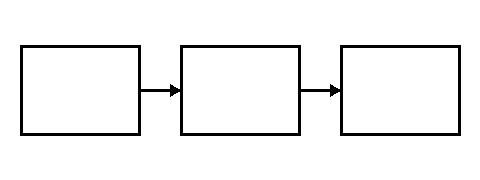
\includegraphics[width=0.65\linewidth]{figuras/fluxo-exemplo.png}
\end{ufcobjeto}

As Figuras~\ref{fig:media}, \ref{fig:larga} e~\ref{fig:png-fluxo} exercitam larguras progressivamente maiores, composição sintética e inclusão de imagem raster sem alterar a API pública do objeto.

\subsection{Gráfico e quadro}

\legend{grafico}{Distribuição sintética de três categorias em arquivo JPEG}
\ufcfonte{Elaboração própria.}
\ufcnota{Valores meramente ilustrativos.}
\label{graf:barras}
\begin{ufcobjeto}[here]
  \centering
  \includegraphics[width=9cm]{figuras/grafico-exemplo.jpg}
\end{ufcobjeto}

O Gráfico~\ref{graf:barras} valida a inclusão de JPEG, a numeração de gráficos e sua presença na Lista de Ilustrações.

\legend{quadro}{Comparação de configurações editoriais do exemplo}
\ufcfonte{Elaboração própria.}
\label{qua:configuracoes}
\begin{ufcobjeto}[here]
  \centering
  \begin{tabular}{lll}
    \hline
    Elemento & Variação A & Variação B \\
    \hline
    Figura & estreita & larga \\
    Código & sem linhas & com linhas \\
    Algoritmo & sem linhas & com linhas \\
    \hline
  \end{tabular}
\end{ufcobjeto}

O Quadro~\ref{qua:configuracoes} exercita conteúdo textual tabular, distinto de uma tabela numérica.

\subsection{Tabela com estilo tabularray-abnt}

\begin{table}[htbp]
\centering
\begin{tallabnttblr}
[
  caption={Indicadores sintéticos com linhas alternadas},
  label={tab:zebra},
  remark{Fonte}={Elaboração própria.},
  remark{Nota}={A alternância de fundo é opcional e usada aqui apenas como exemplo editorial.},
]
{
  colspec={X[l] X[c] X[r]},
  row{even}={bg=black!5},
}
\toprule
Indicador & Ano & Valor \\
\midrule
Alfa & 2024 & 10 \\
Beta & 2025 & 12 \\
Gama & 2026 & 15 \\
Delta & 2026 & 18 \\
\bottomrule
\end{tallabnttblr}
\end{table}

A Tabela~\ref{tab:zebra} complementa a tabela nativa da Seção~\ref{sec:metodologia} e exerce o módulo \texttt{tabularray-abnt} habilitado no documento principal.

\subsection{Código-fonte em diferentes linguagens}

\lstset{language=Python,numbers=left,stepnumber=1,numbersep=8pt}
\legend{codigo}{Função de média em Python com números de linha}
\ufcfonte{Elaboração própria.}
\label{cod:python-numerado}
\begin{ufclisting}[here]
def media(valores):
    return sum(valores) / len(valores)
\end{ufclisting}

\lstset{language=C++,numbers=none}
\legend{codigo}{Função de máximo em C++ sem números de linha}
\ufcfonte{Elaboração própria.}
\label{cod:cpp-sem-numero}
\begin{ufclisting}[here]
int maximo(int a, int b) {
    return a > b ? a : b;
}
\end{ufclisting}

\legend{codigo}{Arquivo Python externo com números de linha}
\ufcfonte{Elaboração própria.}
\label{cod:python-externo}
\begin{ufcobjeto}[here]
  \ufcinputlisting[language=Python,numbers=left,numbersep=8pt]{figuras/exemplo.py}
\end{ufcobjeto}

\lstset{language=Java,numbers=left,stepnumber=2,numbersep=8pt}
\legend{codigo}{Método Java com numeração a cada duas linhas}
\ufcfonte{Elaboração própria.}
\label{cod:java}
\begin{ufclisting}[here]
static int dobro(int valor) {
    int resultado = 2 * valor;
    return resultado;
}
\end{ufclisting}
\lstset{numbers=none,stepnumber=1}

Os Códigos~\ref{cod:python-numerado}, \ref{cod:cpp-sem-numero}, \ref{cod:python-externo} e~\ref{cod:java} demonstram linguagens e políticas de numeração distintas usando o mesmo módulo \texttt{listings}.

\subsection{Algoritmos com e sem números de linha}

\legend{algoritmo}{Máximo divisor comum com números de linha}
\ufcfonte{Elaboração própria.}
\label{alg:mdc-numerado}
\begin{ufcalgoritmo}[here][1]
  \While{$b \neq 0$}
    \State $r \gets a \bmod b$
    \State $a \gets b$
    \State $b \gets r$
  \EndWhile
  \State \Return $a$
\end{ufcalgoritmo}

\legend{algoritmo}{Seleção do maior valor sem números de linha}
\ufcfonte{Elaboração própria.}
\label{alg:maior-sem-numero}
\begin{ufcalgoritmo}[here][0]
  \If{$a > b$}
    \State \Return $a$
  \Else
    \State \Return $b$
  \EndIf
\end{ufcalgoritmo}

Os Algoritmos~\ref{alg:mdc-numerado} e~\ref{alg:maior-sem-numero} validam as duas apresentações de numeração suportadas pelo ambiente.

\subsection{Equação, citação longa e listas}

A Equação~\ref{eq:media-exemplo} exemplifica uma expressão numerada e referenciada no texto.
\begin{equation}
  \bar{x} = \frac{1}{n}\sum_{i=1}^{n}x_i
  \label{eq:media-exemplo}
\end{equation}

Uma citação direta longa também é exercitada no documento de referência:

\Enquote{A composição tipográfica de um documento científico deve ser tratada como parte de um processo reprodutível de edição, revisão e validação, mantendo conteúdo e apresentação suficientemente separados para que mudanças editoriais possam ser verificadas de forma sistemática.}

Exemplo de alíneas e subalíneas:

\begin{ufcalineas}
  \item primeiro item de validação;
  \item segundo item de validação:
    \begin{ufcsubalineas}
      \item subitem de validação.
    \end{ufcsubalineas}
\end{ufcalineas}

Exemplo de enumeração comum:

\begin{enumerate}
  \item preparar o conteúdo;
  \item compilar o documento;
  \item revisar o PDF produzido.
\end{enumerate}
